\documentclass{article}
\usepackage{listings}
\usepackage{hyperref}
\usepackage{url}
\usepackage{graphicx}
\usepackage[letterpaper, hmargin=1.25in, vmargin=1.5in]{geometry}

\title{NPSGD User Guide}
\author{Thomas Dimson\\Natural Phenomenon Simulation Group (NPSG)\\David R. Cheriton School of Computer Science\\University of Waterloo, Canada}

\setlength{\parskip}{0.5\baselineskip}
\newcommand{\mclass}[1]{\texttt{#1}}
\newcommand{\mmethod}[1]{\texttt{#1}}
\lstset{ %
    language=Python,                % choose the language of the code
    showspaces=false,               % show spaces adding particular underscores
    showstringspaces=false,         % underline spaces within strings
    showtabs=false,                 % show tabs within strings adding particular underscores
    breaklines=true,                % sets automatic line breaking
    breakatwhitespace=false,        % sets if automatic breaks should only happen at whitespace
    basicstyle=\ttfamily
}

\begin{document}
\maketitle
\begin{abstract}
    NPSGD is an online framework that makes it easy for researchers to exhibit
    their models online. This document provides a general overview of how the
    system works along with some administration pointers. Notably, it does
    not address the inner workings of how to create models as this is
    documented in the guide called ``Adding a new model to NPSGD''.
\end{abstract}
\tableofcontents

\section{System Requirements}
\label{sec:requirements}
A basic configuration will require:
\begin{itemize}
    \item Python 2.5 or higher (\url{http://www.python.org/})
    \item The Tornado Web server for Python (\url{http://www.tornadoweb.org/})
    \item \LaTeX\ distribution of some form.
    \item UNIX-like operating system. NPSGD has been tested on Ubuntu Linux 9.04
    and 10.04 but should work on other Linux or BSD based platforms.
\end{itemize}

The software has very low hardware requirements. It has been stress tested on 
a single CPU virtual machine with 384 megabytes of RAM. 

\section{System Overview}

\begin{figure}[ht]
    \centering
    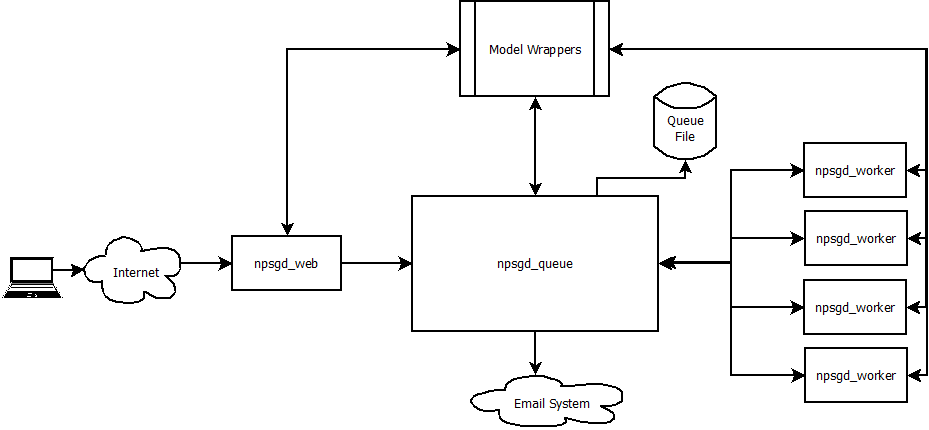
\includegraphics[width=6in]{npsgd_layout.png}
    \caption{Information Flow in NPSGD}
    \label{fig:layout}
\end{figure}

Figure \ref{fig:layout} shows a high level overview of the information flow
within NPSGD. This shows the only client facing daemon, \texttt{npsgd\_web}
serving requests to the user directly. All daemons have a dependency on the
model wrappers and thus the source must be synced between them. As a request is
populated, it is flowed to a disk-backed queue which is polled periodically by
the workers. Once a worker completes a request, it will notify the user via
e-mail.

\subsection{Daemons}
NPSGD is a distributed system which communicates internally and externally via
HTTP. One of the design goals of the system was to allow multiple machines to
perform as workers to avoid to overloading any particular system. To
facilitate this, the framework is split into three daemons:
\begin{itemize}
    \item \texttt{npsgd\_web}: The frontend to NPSGD. The job of this daemon is
    to communicate with all external clients over HTTP. Since no state is kept
    inside the daemon, there is no limit to the number of frontends that exist (though one
    should be sufficient unless you are under heavy load). By default, a
    client visiting \url{http://localhost:8000} will hit this daemon.

    \item \texttt{npsgd\_queue}: The manager of NPSGD. The job of this daemon is
    to keep track of the state of particular model runs, send out e-mail
    confirmations, and to distribute jobs to worker machines. There can only
    ever be one queue within an NPSGD system. By default, it runs on port 9000
    but should not be accessed externally (in particular, it should be
    firewalled off). The queue is a listener for other requests with the 
    \texttt{npsgd\_web} and \texttt{npsgd\_queue} daemons communicating directly
    with the queue via http over port 9000.

    \item \texttt{npsgd\_worker}: The model processor of NPSGD. The job of these
    daemons are to poll the queue for model requests and process them.
    Generally, this takes the form of a finite state machine that spawns some
    external process to actually perform the scientific simulation. After
    processing, it sends results to the requestor's e-mail address.
\end{itemize}

If NPSGD is being configured for long term access, all of these daemons should
have startup scripts associated on the end machine. Sample scripts are available
in the \path{startup/} directory alongside the NPSGD distribution.

Internal communication between daemons is performed over HTTP. Parameters are passed via URL-encoded
JSON that is present in the body of requests for POST requests, and as
parameters for GET requests. For detailed information on the structure of
internal requests, please see their implementations in \path{npsgd_web.py},
\path{npsgd_queue.py} and \path{npsgd_worker.py}. Additionally, 
there is a ``secret'' that is passed in plaintext along every HTTP request communicating with the queue.
A secret is a string, specified in the config file, that must match on both client and queue. This
is \textbf{not} a substitute for a firewall. The queue should be configured to only accept traffic
on port 9000 from known hosts (those that run \texttt{npsgd\_web} and \texttt{npsgd\_worker}).


Each model that is implemented for NPSGD must be available for the queue, the
web frontend and the worker machines. A NFS mount for the models is particularly
handy for this purpose (though not necessary).

\subsection{Request Flow}
A sample model of NPSGD is available at
\url{http://www.npsg.uwaterloo.ca/models/ABMU.php}. It would be helpful to try
this out in order to gain understanding of the system. The typical request flow
would be something like this:
\begin{enumerate}
    \item User visits the model site via \url{http://localhost:8000/models/example},
    which is served using \texttt{npsgd\_web}.

    \item User submits a request for the example model, \texttt{npsgd\_web}
    acquires a confirmation code from \texttt{npsgd\_queue}.

    \item \texttt{npsgd\_queue} e-mails the same confirmation code to the user's e-mail
    address.
    
    \item User clicks the link in the e-mail, usually something like
    \url{http://localhost:8000/confirm\_submission/code}. 

    \item \texttt{npsgd\_web} forwards the confirmation onto
    \texttt{npsgd\_queue}. At this point the model request is ready to be
    processed.

    \item \texttt{npsgd\_worker} has been polling the queue for a task. Since
    now there is a task, it receives a task response.

    \item \texttt{npsgd\_worker} prepares execution, spawns a subprocess to run
    the underlying model.
    
    \item Model execution completes. \texttt{npsgd\_worker} creates a \LaTeX\ 
    document with the results.

    \item \LaTeX\ document and other attachments are sent to the user's e-mail.
    \texttt{npsgd\_worker} tells the \texttt{npsgd\_queue} that it has executed successfully.
\end{enumerate}

\subsection{Fault Tolerance}
NPSGD has been designed to be fault tolerant. Whenever a web request is made,
\texttt{npsgd\_web} will check with the queue to ensure it is up and that it has
workers on the line that have polled for a request recently. If one of these
conditions is not met, a simple error message is displayed to the requester.

When processing a task, \texttt{npsgd\_workers} communicate back to the queue
with a keepalive request to make sure that the queue knows that the worker is
still alive. If this keepalive has not been heard for a long while, the queue
daemon will put the request back at the tail of the queue and increase its failure count.

All requests are tried for a fixed number of times before a complete failure (by
default, the queue will retry a request three times before declaring it failed).
Upon failure, an error message is e-mailed to the user.

If the e-mail system is ever down, \texttt{npsgd\_queue} will keep trying to send e-mails out
until they have successfully completed.

\texttt{npsgd\_queue} can be shut down with no data loss (even if requests are
in the queue).
The queue server is serialized to disk (using Python's \texttt{shelve} standard
module) every time a new request jumps into the
queue or one is taken out. When the queue boots up, it loads back all the
requests that had confirmation codes or had model requests in the queue. If
a model has been updated since the queue went down, there will be no way to
complete the request so an e-mail is sent to the requester to notify them of
failure. It is likely that they can simply retry their request at that point.

\section{Software Layout}
NPSGD ships in exactly the same way it was developed and is not easily converted
into a form that matches the standard UNIX layouts. When you clone the main
repository for NPSGD, you will see the following files and directories:
\begin{itemize}
    \item \path{config.example}: An example configuration file for NPSGD.
    \item \path{epydoc.cfg}: Config file for generating an HTML representation
          of the code using epydoc.
    \item \path{LICENSE}: License agreement for distribution.
    \item \path{README}: Easy readme guide to NPSGD.
    \item \path{npsgd\_web.py}: Web daemon for handling client requests.
    \item \path{npsgd\_queue.py}: Daemon for queueing NPSGD model runs.
    \item \path{npsgd\_worker.py}: Worker for actually processing NPSGD model
          runs.
    \item \path{doc/}: Directory containing NPSGD documentation.
    \item \path{models/}: Default directory for storing user-defined models.
    \item \path{npsgd/}: Helper package containing modules required to run the
          daemons.
    \item \path{startup/}: Directory containing some sample startup scripts for
          Ubuntu (must be modified to specify paths correctly).
    \item \path{static/}: Directory containing static files served by the web
          server (Javascript, css).
    \item \path{templates/}: Directory containing templates used by NPSGD.
\end{itemize}

\subsection{Templates}
Templates are used in many different ways within NPSGD:
\begin{itemize}
    \item To create the HTML that is served by the web daemon.
    \item To create the e-mail sent by the queue and worker daemons.
    \item To create \LaTeX\ markup to send results to the user.
\end{itemize}

All templates for NPSGD are stored in the \path{templates/} subdirectory. This
is meant to be user defined. The default templates shipped with NPGSD are 
specific to the models within the Natural Phenomenon Simulation Group and are
intended to be used as a guide for other NPSGD users.

Templates use a syntax created for the Tornado web server. This syntax is
documented at the Tornado site: \url{http://www.tornadoweb.org/}, under
templates.

\subsubsection{HTML Templates}
NPSGD ships with two sets of HTML templates, one for an embedded site (served
directly without entities like title tags), and one for a basic site. These
templates are used by the web daemon to display HTML directly to the user. Both are
available under the \path{templates/html/} subdirectory. These files contain:
\begin{enumerate}
    \item \texttt{base.html}: Template that all other templates inherit from.
    It could contain entities like HTML headers and footers.

    \item \texttt{model.html}: The template that displays a model to the user.

    \item \texttt{model\_error.html}: The template that displays a message when
    an error occurs in the model.

    \item \texttt{confirm.html}: Template that displays after a model request has
    been made (displays that an e-mail will be dispatched to the user).

    \item \texttt{confirmed.html}: Template that displays after a confirmation code
    has been entered correctly.

    \item \texttt{already\_confirmed.html}: Template that displays after a
    confirmation code has been entered for a second time (displays a
    message saying that the model will not be rerun).
\end{enumerate}

\subsubsection{Email Templates}
Emails are used as communication to the user after a request has been performed
via HTML. Each template comes in two parts: one for the email subject, and one
for the email body. The naming convention is ``name\_body.txt'' for body and
``name\_subject.txt'' for subject. In particular, these templates are available:
\begin{itemize}
    \item \texttt{results\_email}: The email used to display model run results.
    \item \texttt{failure\_email}: The email used to notify the user when a
    certain error threshold has been met during across model execution attempts.
    \item \texttt{confirm\_email}: The email used to communicate the
    confirmation code for a particular model request.
    \item \texttt{confirmation\_failed\_email}: The email that is used to
    communicate that a confirmation code has expired prematurely. This is only
    sent if the user receives a confirmation code, the queue goes down, then
    comes up with different model versions.
    \item \texttt{lost\_task\_email}: The email that is used to communicate that
    we are no longer able to execute a particular model request. This is sent
    only if we are processing a model request, the queue goes down and then
    comes up with different model versions.
\end{itemize}

\subsubsection{\LaTeX\ Templates}
There is only one LaTeX template, namely \path{result\_template.tex}. This is
used to declare all the packages required for a model results PDF. Inside, there
is an empty variable where the details of a model run will go. Models themselves
specify the model details, but it is always wrapped in this template.


\section{Development Environment}
Since NPSGD consists of so many components, creating a quick development
environment may seem overwhelming. First of all, ensure that all the 
requirements mentioned in Section \ref{sec:requirements} are installed. 
After that, clone NPSGD from the
main development site and create a custom copy of the config file:
\begin{verbatim}
git clone git://github.com/cosbynator/NPSGD.git
cp config.example config.cfg
\end{verbatim}

The config file will need a few changes to run, notably:
\begin{itemize}
    \item Change \texttt{npsgbase} to point at the directory that you cloned the
    software into (e.g., \path{/home/tdimson/npsgd}).
    \item Change \texttt{pdflatexPath} to point at your \texttt{pdflatex}
    binary.
    \item Change the \texttt{email} section to specify a valid
    username/password and to enter your SMTP server. E-mail uses the SMTP protocol
    and has configuration
    options for toggling various SMTP features (notably encryption and
    SMTPAUTH). The defaults are set up for a gmail 
    account (provided you specify a valid username/password). Any provider
    supporting SMTP should be compatible with NPSGD.
    \item Change \texttt{matlabPath} if you will be testing/editing Matlab
    models.
\end{itemize}

After completing these sections you will be able to run all three daemons on a
local terminal. Specifically, run the following in separate terminal windows:
\begin{verbatim}
python npsgd_web.py
python npsgd_queue.py
python npsgd_worker.py
\end{verbatim}
Logging will be printed to standard error unless otherwise specified (using the
\texttt{-l} command line option). After
running \texttt{npsgd\_web} you should be able to browse to
\url{http://localhost:8000/models/example} and see some sample output. Try
performing a complete model run to make sure the system is operating correctly.

\section{A word on models}
Models are the key component to customizing NPSGD. The scope of this document
does not cover the \textit{implementation} of custom models (see ``Adding a new
model to NPSGD'' from \url{http://www.npsg.uwaterloo.ca} for that). Still, it is important to understand how they fit
into the system.

Models are Python files that inherit from \mclass{ModelTask} in
order to provide complete flexibility for underlying implementation. These
Python files often act as wrappers to existing models that are implemented in
some other language (we have models implemented in both Matlab and C++). 
This does not force the model implementation to be in Python;
Python acts as a facilitator between NPSGD and the underyling model. 

Each daemon is configured to monitor the model directory, by default under
\path{models/}. Python files in this directory act as ``plugins'' to the system
- models are implemented in them. The daemons periodically scan the directory
and look at the all the python files, those that inherit from \mclass{ModelTask}
are imported into the system. When importing, a hash of the file is used to tag
the model with a ``version''. Duplicate versions of models are ignored (not
imported into the system), while new versions are stored. Old versions are
retained in the system in case there are any queued requests that are still
acting on the old version. For this reason, it is important for the developer to 
reload the page after updating any models if they wish to test the new version.

Models are self-contained: they have all the information necessary for the
queue, web and worker daemons to operate. In particular, they contain the
parameters necessary for the web interface to configure the models and the
execution cycle necessary in order for the workers to run a model with a
particular parameter set. The code for the models must be shared
across the daemons: this is done manually, or via a NFS mount.


\section{Static Files}
In addition to templates, NPSGD needs the use of certain static files to
customize the in-browser behaviour. All static files are available in the
\path{static/} subdirectory.

\subsection{Javascript}
NPSGD uses Javascript to handle parameter verification and provide UI
widgets for the user. The following are located in the \path{static/js}
subdirectory:
\begin{enumerate}
    \item \texttt{npsgd.js}: Our particular javascript files.
    \item \texttt{jquery-version.min.js}: JQuery, a javascript library that
    makes writing javascript simpler: \url{http://jquery.com/}
    \item \texttt{jquery.qtip.min.js}: A library for creating popup tooltips.
    This is used for model's helper text.
    \url{http://craigsworks.com/projects/qtip/}
    \item \texttt{jquery-ui-version.min.js}: JQuery UI, a set of UI widgets for
    JQuery: \url{http://jqueryui.com/}. This is used to provide an interface for 
    widgets such as sliders and range selectors.
    \item \texttt{jquery.validate.min.js}: JQuery validation plugin. This is
    used to perform parameter verification in client side, before requests are sent
    to the server:
    \url{http://bassistance.de/jquery-plugins/jquery-plugin-validation/}
\end{enumerate}

\subsection{CSS}
In addition to Javascript, some basic CSS needs to be shared across all
templates. These are in the \path{static/css} subdirectory.
\begin{enumerate}
    \item \texttt{npsgd.css}: This provides just a couple of CSS includes that
    are needed across all templates.
    \item \texttt{smoothness/}: This subdiretory contains the default CSS files
    for the JQuery UI project. It is used to dislay the widgets of JQuery UI.
\end{enumerate}

\subsection{Images}
Finally, there are some images that NPSGD needs to display available in the
\path{static/images} subdirectory. 

\end{document}
